\titre{Opérateurs} : $== \; ; \; > \; ; \; < \; ; \; >= \; ; \; <= \; ; \; != \; ; \; \&\& \; ; \; || \; ; \; !$

\par

\titre{Valeurs booléennes} 
\begin{itemize}
	\item 0 = faux
	\item 1 ou autre valeur = vrai
\end{itemize}

\par

\titre{Condition} \\
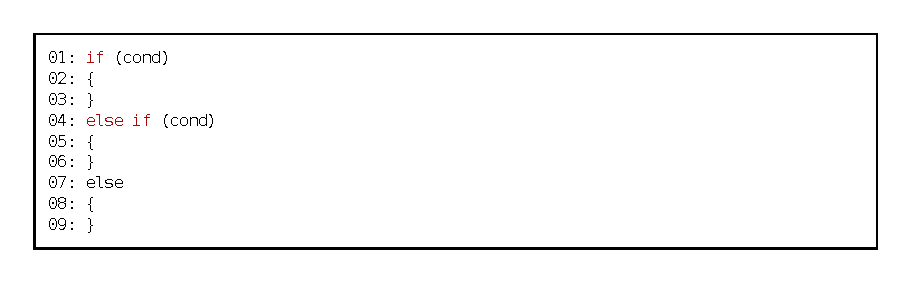
\includegraphics[width=\linewidth]{D6_1.pdf}

\par

\titre{Switch} \\
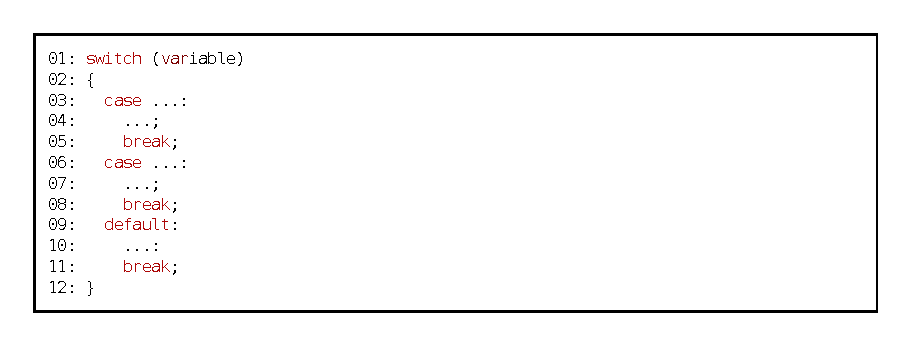
\includegraphics[width=\linewidth]{D6_2.pdf}

\par

\titre{Ternaire} \\
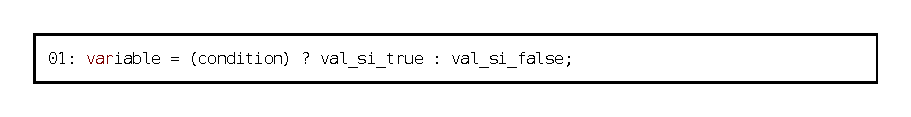
\includegraphics[width=\linewidth]{D6_3.pdf}

\vspace{-0.5cm}
